\documentclass[12pt]{article}

\usepackage[a4paper,margin=1in]{geometry}
\usepackage{amsmath,amssymb}
\usepackage{newtxtext,newtxmath} % Times-style font
\usepackage{fancyhdr}
\usepackage{listings}
\usepackage{graphicx}
\usepackage{float}
\usepackage{algorithm}
\usepackage{algpseudocode}
\usepackage{xcolor}
\usepackage{booktabs}
\usepackage{array}

\setlength{\textfloatsep}{10pt}
\setlength{\floatsep}{10pt}

\setlength{\parindent}{0pt}
\setlength{\parskip}{5pt}

% Keep entire document at 12 pt
\AtBeginDocument{
    \fontsize{12pt}{14pt}\selectfont
}

\lstdefinestyle{code}{
    language=Python,
    basicstyle=\ttfamily\fontsize{10pt}{12pt}\selectfont,
    breaklines=true,
    breakatwhitespace=false,
    frame=single,
    numbers=left,
    numberstyle=\tiny\color{gray},
    keywordstyle=\color{blue},
    commentstyle=\color{gray},
    stringstyle=\color{green!50!black},
    columns=fullflexible,
    keepspaces=true,
    showstringspaces=false
}

\lstdefinestyle{output}{
    basicstyle=\ttfamily\fontsize{10pt}{12pt}\selectfont,
    breaklines=true,
    breakatwhitespace=false,
    frame=single,
    numbers=none,
    backgroundcolor=\color{gray!4},
    columns=fullflexible,
    keepspaces=true,
    showstringspaces=false
}

% ------------------------------------------------
% Header
% ------------------------------------------------

\pagestyle{fancy}
\fancyhf{}

\fancyhead[L]{Name: Kishan Sahu{\hspace{6cm}}}
\fancyhead[R]{Enrollment No.: P26DS017}

\renewcommand{\headrulewidth}{0.4pt}
\setlength{\headheight}{15pt}

\begin{document}

% ------------------------------------------------
% TITLE
% ------------------------------------------------

\begin{center}
\textbf{Computer Science and Engineering Department, SVNIT, Surat}\\
\textbf{M.Tech. I -- Semester I}\\
\textbf{Computer Vision and Image Processing (CSCS111/CSDS119)}\\
\textbf{Lab Assignment 6}\\
\textbf{Image Segmentation}
\end{center}
\vspace{-4pt}
\hrule
\vspace{4pt}

% ------------------------------------------------
% SECTION 1: INTRODUCTION
% ------------------------------------------------
\section{Introduction and Problem Statement}

Image segmentation is a foundational task in computer vision aimed at partitioning a digital image into multiple meaningful, visually distinct regions corresponding to objects or structural boundaries. This laboratory assignment explores both classical spatial segmentation approaches and advanced composite pipelines using a real-world photograph (\texttt{cup\_holding.jpg}) of a person holding an object.

The objectives are structured into two distinct parts:
\begin{enumerate}
    \item \textbf{PART A}:
    \begin{itemize}
        \item Detect prominent isolated points and directional lines ($0^\circ, 90^\circ, +45^\circ, -45^\circ$) using spatial convolution masks.
        \item Detect object and human boundaries using spatial edge detection operators: Roberts Cross, Prewitt, Sobel, and Laplacian.
        \item Segment the image into foreground and background using Iterative Global Thresholding and Otsu's optimal thresholding.
        \item Implement Region Growing segmentation and systematically analyze the impact of seed point placement and similarity criteria ($\Delta T$).
        \item Conduct a rigorous comparative evaluation on the relative efficacy of each technique.
    \end{itemize}
    \item \textbf{PART B}:
    \begin{itemize}
        \item Design and implement a composite segmentation pipeline to isolate and retain the held object—specifically a \textbf{black cup} (intensity values $\approx 30\text{--}70$) held against a \textbf{gray background} ($\approx 200\text{--}245$) and hand skin tones ($\approx 150\text{--}210$).
        \item Remove the surrounding environment (setting non-cup pixels to clean white), or alternately make the object disappear through inpainting while preserving background and hand posture.
        \item Contrast the pipeline's performance against single-technique thresholding failures (Global Otsu and Naive dark thresholding).
    \end{itemize}
\end{enumerate}

\subsection{Input Image Setup and Preprocessing}
The test image \texttt{cup\_holding.jpg} has dimensions $525 \times 350$ pixels with 3 RGB color channels. The preprocessing block loads the image using OpenCV, converts color representations, and displays the original input.

\begin{lstlisting}[style=code]
import cv2
import numpy as np
import matplotlib.pyplot as plt
from collections import deque

# Load image
img_bgr = cv2.imread('cup_holding.jpg')
img_rgb = cv2.cvtColor(img_bgr, cv2.COLOR_BGR2RGB)
gray = cv2.cvtColor(img_bgr, cv2.COLOR_BGR2GRAY)

print(f"Loaded cup_holding.jpg with dimensions: {img_bgr.shape[1]}x{img_bgr.shape[0]} (Channels: {img_bgr.shape[2]})")

fig, ax = plt.subplots(figsize=(6, 4))
ax.imshow(img_rgb)
ax.set_title("Original Image (cup_holding.jpg)")
ax.axis("off")
plt.tight_layout()
plt.show()
\end{lstlisting}

\begin{lstlisting}[style=output]
Loaded cup_holding.jpg with dimensions: 525x350 (Channels: 3)
\end{lstlisting}

\begin{figure}[H]
    \centering
    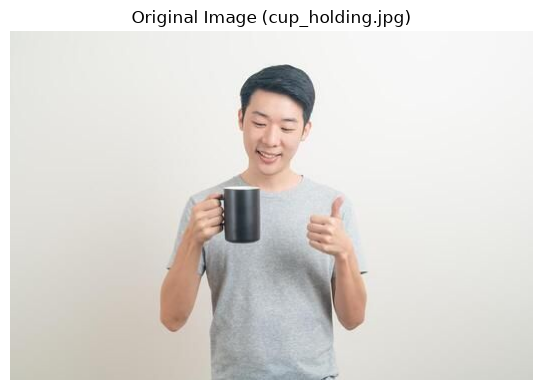
\includegraphics[width=0.65\textwidth]{figures/fig1_original.png}
    \caption{Original input photograph (\texttt{cup\_holding.jpg}) showing a person holding a black cup against a neutral gray background.}
    \label{fig:original}
\end{figure}

% ------------------------------------------------
% SECTION 2: PART A.1 POINT AND LINE DETECTION
% ------------------------------------------------
\section{Part A.1: Point and Directional Line Detection}

Spatial feature detection can be formulated using localized linear convolution filters. Discontinuities in an image are characterized by abrupt intensity changes across spatial neighborhoods.

\subsection{Mathematical Formulation}
\begin{enumerate}
    \item \textbf{Point Detection Mask}: A point discontinuity corresponds to an isolated pixel whose intensity differs substantially from all surrounding neighbors. The $3 \times 3$ isotropic Laplacian mask is defined as:
    \begin{equation}
    K_{\text{point}} = \begin{bmatrix} -1 & -1 & -1 \\ -1 & 8 & -1 \\ -1 & -1 & -1 \end{bmatrix}
    \end{equation}
    A point is classified as prominent if the absolute filtered response exceeds a predetermined threshold: $|R(x, y)| \ge T_{\text{point}}$.

    \item \textbf{Directional Line Masks}: Lines of one-pixel thickness oriented along specific angles are detected using masks where coefficients along the preferred direction are positive and orthogonal coefficients are negative:
    \begin{align}
    K_{\text{H}} &= \begin{bmatrix} -1 & -1 & -1 \\ 2 & 2 & 2 \\ -1 & -1 & -1 \end{bmatrix}, &
    K_{\text{V}} &= \begin{bmatrix} -1 & 2 & -1 \\ -1 & 2 & -1 \\ -1 & 2 & -1 \end{bmatrix}, \\
    K_{+45^\circ} &= \begin{bmatrix} -1 & -1 & 2 \\ -1 & 2 & -1 \\ 2 & -1 & -1 \end{bmatrix}, &
    K_{-45^\circ} &= \begin{bmatrix} 2 & -1 & -1 \\ -1 & 2 & -1 \\ -1 & -1 & 2 \end{bmatrix}
    \end{align}
\end{enumerate}

\subsection{Python Implementation}
\begin{lstlisting}[style=code]
# Point detection kernel
point_kernel = np.array([[-1, -1, -1],
                         [-1,  8, -1],
                         [-1, -1, -1]], dtype=np.float32)
point_resp = np.abs(cv2.filter2D(gray, cv2.CV_32F, point_kernel))
# Prominent point detection threshold (top 0.5% responses)
point_thresh = np.percentile(point_resp, 99.5)
point_detected = (point_resp > point_thresh).astype(np.uint8) * 255

# Directional line detection kernels
line_h = np.array([[-1, -1, -1],
                   [ 2,  2,  2],
                   [-1, -1, -1]], dtype=np.float32)
line_v = np.array([[-1,  2, -1],
                   [-1,  2, -1],
                   [-1,  2, -1]], dtype=np.float32)
line_p45 = np.array([[-1, -1,  2],
                     [-1,  2, -1],
                     [ 2, -1, -1]], dtype=np.float32)
line_m45 = np.array([[ 2, -1, -1],
                     [-1,  2, -1],
                     [-1, -1,  2]], dtype=np.float32)

resp_h = np.abs(cv2.filter2D(gray, cv2.CV_32F, line_h))
resp_v = np.abs(cv2.filter2D(gray, cv2.CV_32F, line_v))
resp_p45 = np.abs(cv2.filter2D(gray, cv2.CV_32F, line_p45))
resp_m45 = np.abs(cv2.filter2D(gray, cv2.CV_32F, line_m45))
\end{lstlisting}

\begin{figure}[H]
    \centering
    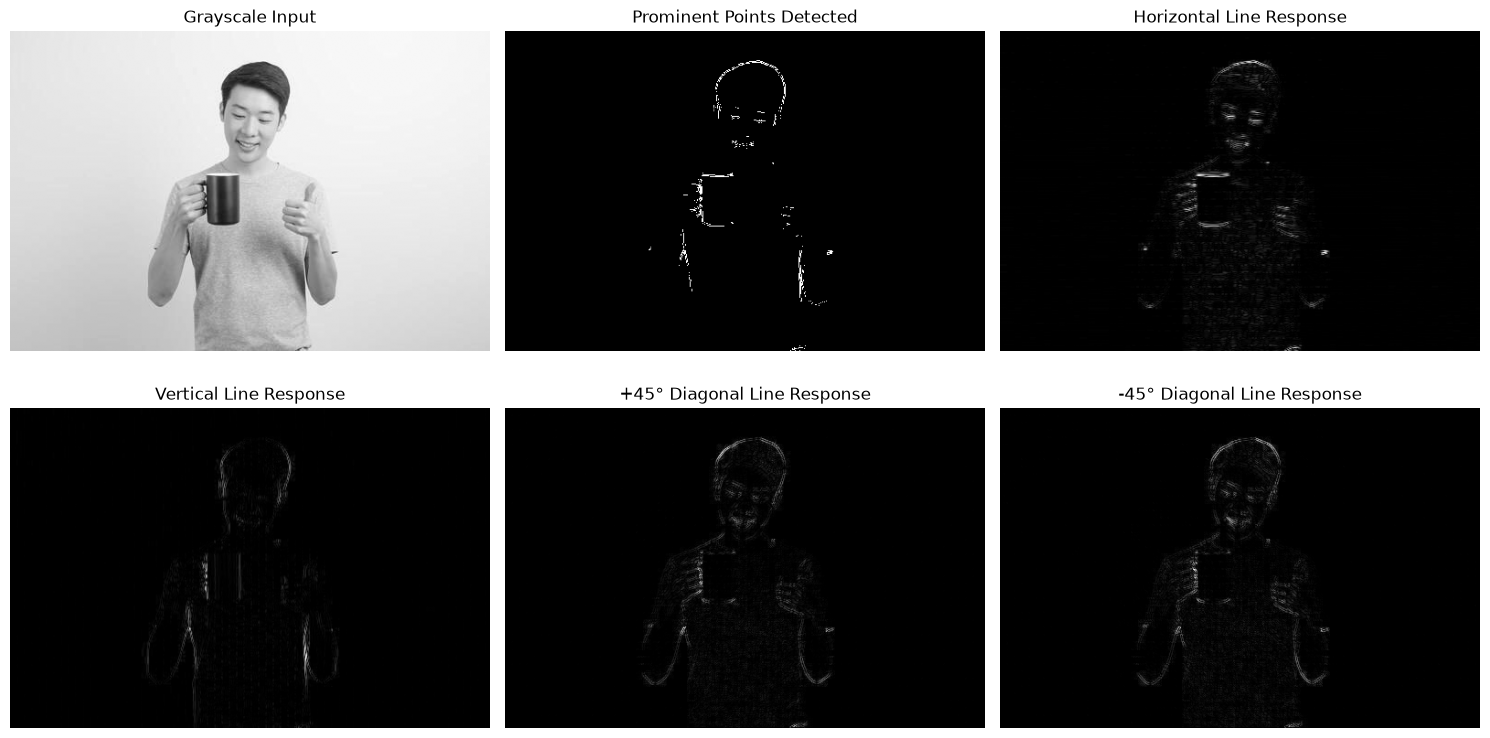
\includegraphics[width=\textwidth]{figures/fig2_point_line.png}
    \caption{Visual responses for prominent point detection and directional line detection ($0^\circ$, $90^\circ$, $+45^\circ$, and $-45^\circ$).}
    \label{fig:point_line}
\end{figure}

\textbf{Analysis}: The point detection mask isolates high-frequency texture anomalies, highlights on the cup rim, and specular reflection spots. The directional line masks selectively amplify linear structures along the specified angle; for instance, the horizontal mask accentuates the shoulders and top of the cup rim, whereas the vertical mask accentuates the sides of the cup and the human torso silhouette. However, line masks produce discontinuous segments and cannot form closed object boundaries.

% ------------------------------------------------
% SECTION 3: PART A.2 EDGE DETECTION OPERATORS
% ------------------------------------------------
\section{Part A.2: Edge Detection Operators}

Edge detection computes spatial gradient approximations to locate boundaries between regions of contrasting intensity.

\subsection{Mathematical Formulation}
\begin{enumerate}
    \item \textbf{Roberts Cross ($2 \times 2$)}: Computes diagonal finite differences:
    \begin{equation}
    R_x = \begin{bmatrix} 1 & 0 \\ 0 & -1 \end{bmatrix}, \quad R_y = \begin{bmatrix} 0 & 1 \\ -1 & 0 \end{bmatrix}, \quad |\nabla f| \approx \sqrt{G_x^2 + G_y^2}
    \end{equation}
    \item \textbf{Prewitt Operator ($3 \times 3$)}: Uses orthogonal finite differences with equal neighbor weighting:
    \begin{equation}
    P_x = \begin{bmatrix} -1 & 0 & 1 \\ -1 & 0 & 1 \\ -1 & 0 & 1 \end{bmatrix}, \quad P_y = \begin{bmatrix} -1 & -1 & -1 \\ 0 & 0 & 0 \\ 1 & 1 & 1 \end{bmatrix}
    \end{equation}
    \item \textbf{Sobel Operator ($3 \times 3$)}: Incorporates Gaussian smoothing across the center row/column:
    \begin{equation}
    S_x = \begin{bmatrix} -1 & 0 & 1 \\ -2 & 0 & 2 \\ -1 & 0 & 1 \end{bmatrix}, \quad S_y = \begin{bmatrix} -1 & -2 & -1 \\ 0 & 0 & 0 \\ 1 & 2 & 1 \end{bmatrix}
    \end{equation}
    \item \textbf{Laplacian Operator}: Isotropic second-derivative operator capturing zero-crossings:
    \begin{equation}
    \nabla^2 f = \frac{\partial^2 f}{\partial x^2} + \frac{\partial^2 f}{\partial y^2}, \quad L = \begin{bmatrix} 0 & 1 & 0 \\ 1 & -4 & 1 \\ 0 & 1 & 0 \end{bmatrix}
    \end{equation}
\end{enumerate}

\subsection{Python Implementation}
\begin{lstlisting}[style=code]
# Roberts Cross
rob_x = np.array([[1, 0], [0, -1]], dtype=np.float32)
rob_y = np.array([[0, 1], [-1, 0]], dtype=np.float32)
gx_rob = cv2.filter2D(gray, cv2.CV_32F, rob_x)
gy_rob = cv2.filter2D(gray, cv2.CV_32F, rob_y)
roberts = np.sqrt(gx_rob**2 + gy_rob**2)

# Prewitt
prew_x = np.array([[-1, 0, 1], [-1, 0, 1], [-1, 0, 1]], dtype=np.float32)
prew_y = np.array([[-1, -1, -1], [0, 0, 0], [1, 1, 1]], dtype=np.float32)
gx_prew = cv2.filter2D(gray, cv2.CV_32F, prew_x)
gy_prew = cv2.filter2D(gray, cv2.CV_32F, prew_y)
prewitt = np.sqrt(gx_prew**2 + gy_prew**2)

# Sobel
sobel_x = cv2.Sobel(gray, cv2.CV_32F, 1, 0, ksize=3)
sobel_y = cv2.Sobel(gray, cv2.CV_32F, 0, 1, ksize=3)
sobel = np.sqrt(sobel_x**2 + sobel_y**2)

# Laplacian (2nd Derivative)
laplacian = np.abs(cv2.Laplacian(gray, cv2.CV_32F, ksize=3))
\end{lstlisting}

\begin{figure}[H]
    \centering
    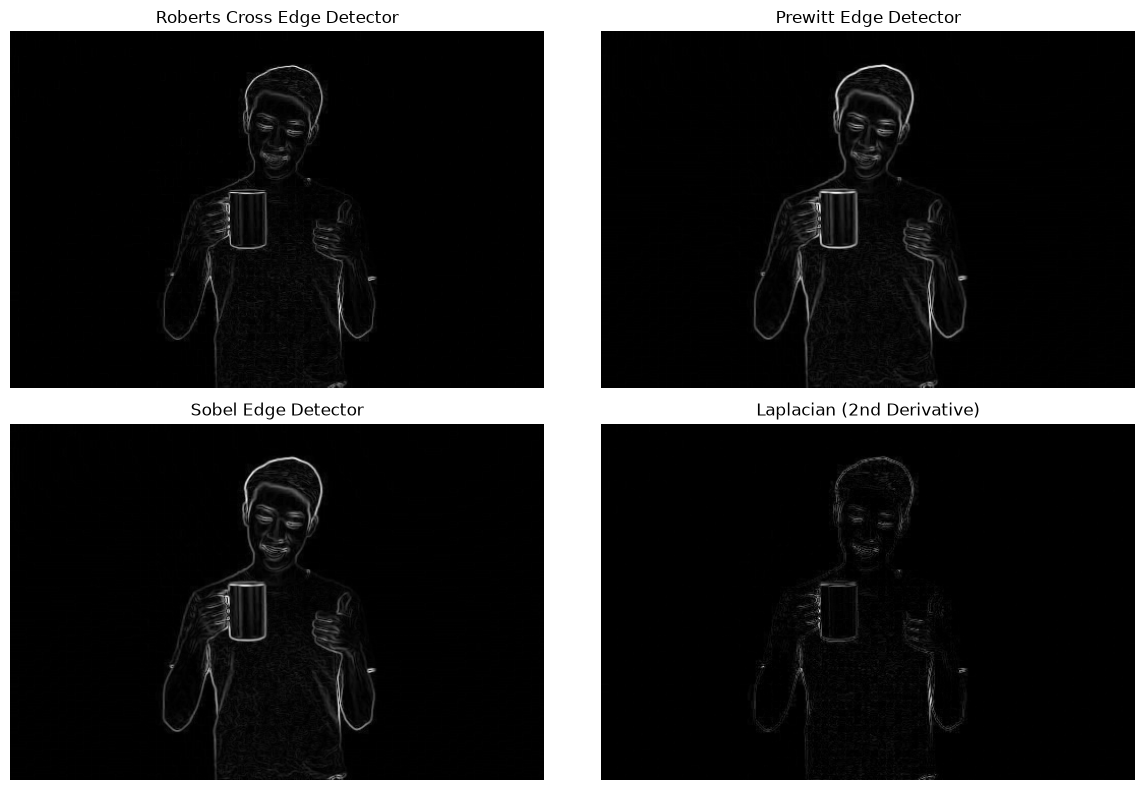
\includegraphics[width=0.92\textwidth]{figures/fig3_edges.png}
    \caption{Comparison of spatial edge detection operators: Roberts Cross, Prewitt, Sobel, and Laplacian.}
    \label{fig:edges}
\end{figure}

\textbf{Analysis}:
\begin{itemize}
    \item \textbf{Roberts Cross}: Employs a tiny $2\times 2$ stencil. It exhibits the thinnest edge responses but is severely degraded by local pixel noise.
    \item \textbf{Prewitt vs. Sobel}: Both use $3\times 3$ neighborhoods, yet Sobel provides significantly smoother, more continuous edges because the central coefficient ($2$) incorporates localized triangular/Gaussian smoothing.
    \item \textbf{Laplacian}: As a second-derivative operator, it generates distinct double-edge artifacts and amplifies high-frequency noise across the background.
\end{itemize}

% ------------------------------------------------
% SECTION 4: PART A.3 THRESHOLDING
% ------------------------------------------------
\section{Part A.3: Thresholding-Based Segmentation}

Thresholding segments an image by partitioning its intensity histogram into binary classes: foreground ($G_1$) and background ($G_2$).

\subsection{Mathematical Formulation}
\begin{enumerate}
    \item \textbf{Iterative Global Thresholding}:
    An initial estimate $T_0 = \frac{1}{MN}\sum_{x,y} f(x, y)$ is iteratively refined:
    \begin{equation}
    m_1 = \frac{1}{|G_1|} \sum_{(x,y) \in G_1} f(x, y), \quad m_2 = \frac{1}{|G_2|} \sum_{(x,y) \in G_2} f(x, y), \quad T_{k+1} = \frac{m_1 + m_2}{2}
    \end{equation}
    The loop terminates when $|T_{k+1} - T_k| < \epsilon$ (with $\epsilon = 0.5$).

    \item \textbf{Otsu's Thresholding}:
    Selects $T^*$ that maximizes the between-class variance $\sigma_B^2(T)$:
    \begin{equation}
    \sigma_B^2(T) = \omega_0(T) \omega_1(T) [\mu_0(T) - \mu_1(T)]^2
    \end{equation}
    where $\omega_0, \omega_1$ denote cumulative class probabilities and $\mu_0, \mu_1$ denote class means up to threshold $T$.
\end{enumerate}

\subsection{Python Implementation and Results}
\begin{lstlisting}[style=code]
# Iterative Global Thresholding
T = float(gray.mean())
while True:
    g1 = gray[gray > T]
    g2 = gray[gray <= T]
    m1 = g1.mean() if len(g1) > 0 else 0
    m2 = g2.mean() if len(g2) > 0 else 0
    new_T = (m1 + m2) / 2
    if abs(T - new_T) < 0.5:
        break
    T = new_T

global_thresh_val = T
global_seg = (gray > global_thresh_val).astype(np.uint8) * 255

# Otsu's Thresholding
otsu_thresh_val, otsu_seg = cv2.threshold(gray, 0, 255, cv2.THRESH_BINARY + cv2.THRESH_OTSU)

print(f"Iterative Global Threshold: {global_thresh_val:.2f}")
print(f"Otsu Optimal Threshold:    {otsu_thresh_val:.2f}")
\end{lstlisting}

\begin{lstlisting}[style=output]
Iterative Global Threshold: 187.13
Otsu Optimal Threshold:    186.00
\end{lstlisting}

\begin{figure}[H]
    \centering
    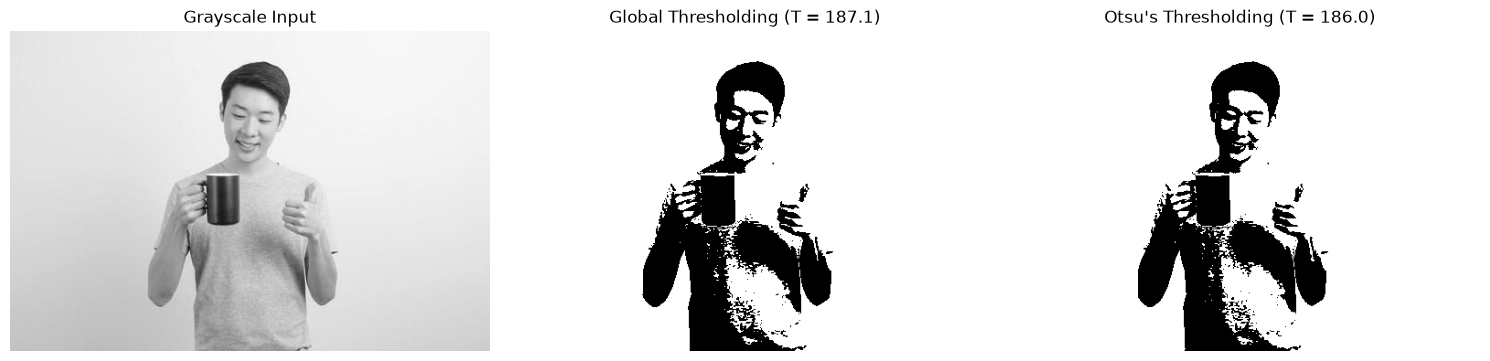
\includegraphics[width=\textwidth]{figures/fig4_thresholding.png}
    \caption{Thresholding comparison: Grayscale input, Iterative Global Thresholding ($T=187.1$), and Otsu's optimal thresholding ($T=186.0$).}
    \label{fig:thresholding}
\end{figure}

\textbf{Analysis}: Both algorithms converge to nearly identical partition thresholds ($187.13$ vs. $186.00$). While both succeed in separating the bright gray background from the darker person, \textbf{neither method can isolate the black cup alone} because global thresholding bisects the histogram into only two broad classes, grouping the cup, hand, and torso into a single foreground mass.

% ------------------------------------------------
% SECTION 5: PART A.4 REGION GROWING
% ------------------------------------------------
\section{Part A.4: Region-Based Segmentation (Region Growing)}

Region growing is a spatial segmentation technique that groups neighboring pixels into larger regions based on predefined similarity criteria.

\subsection{Algorithm and Similarity Criterion}
Given a seed coordinate $(r_{\text{seed}}, c_{\text{seed}})$, adjacent 4-connected neighbor pixels $(r, c)$ are appended to the region $\mathcal{R}$ if the intensity deviation satisfies:
\begin{equation}
|f(r, c) - f(r_{\text{seed}}, c_{\text{seed}})| \le \Delta T
\end{equation}

\subsection{Python Implementation and Sensitivity Analysis}
\begin{lstlisting}[style=code]
def region_growing(img_gray, seed, threshold=30):
    h, w = img_gray.shape
    segmented = np.zeros((h, w), dtype=bool)
    visited = np.zeros((h, w), dtype=bool)
    
    sr, sc = seed
    seed_val = float(img_gray[sr, sc])
    queue = deque([(sr, sc)])
    visited[sr, sc] = True
    segmented[sr, sc] = True
    
    while queue:
        r, c = queue.popleft()
        for dr, dc in [(-1, 0), (1, 0), (0, -1), (0, 1)]:
            nr, nc = r + dr, c + dc
            if 0 <= nr < h and 0 <= nc < w and not visited[nr, nc]:
                visited[nr, nc] = True
                if abs(float(img_gray[nr, nc]) - seed_val) <= threshold:
                    segmented[nr, nc] = True
                    queue.append((nr, nc))
    return (segmented.astype(np.uint8) * 255)

# Seed 1: Inside Black Cup (row 187, col 230, intensity ~48)
seed_cup = (187, 230)
cup_t15 = region_growing(gray, seed_cup, threshold=15)
cup_t30 = region_growing(gray, seed_cup, threshold=30)
cup_t60 = region_growing(gray, seed_cup, threshold=60)

# Seed 2: On Gray Background (row 50, col 50, intensity ~225)
seed_bg = (50, 50)
bg_t30 = region_growing(gray, seed_bg, threshold=30)
\end{lstlisting}

\begin{lstlisting}[style=output]
Seed at Cup (187, 230) with ΔT=15 -> Segmented Pixels: 442
Seed at Cup (187, 230) with ΔT=30 -> Segmented Pixels: 958
Seed at Cup (187, 230) with ΔT=60 -> Segmented Pixels: 1724
Seed at Background (50, 50) with ΔT=30 -> Segmented Pixels: 139457
\end{lstlisting}

\begin{figure}[H]
    \centering
    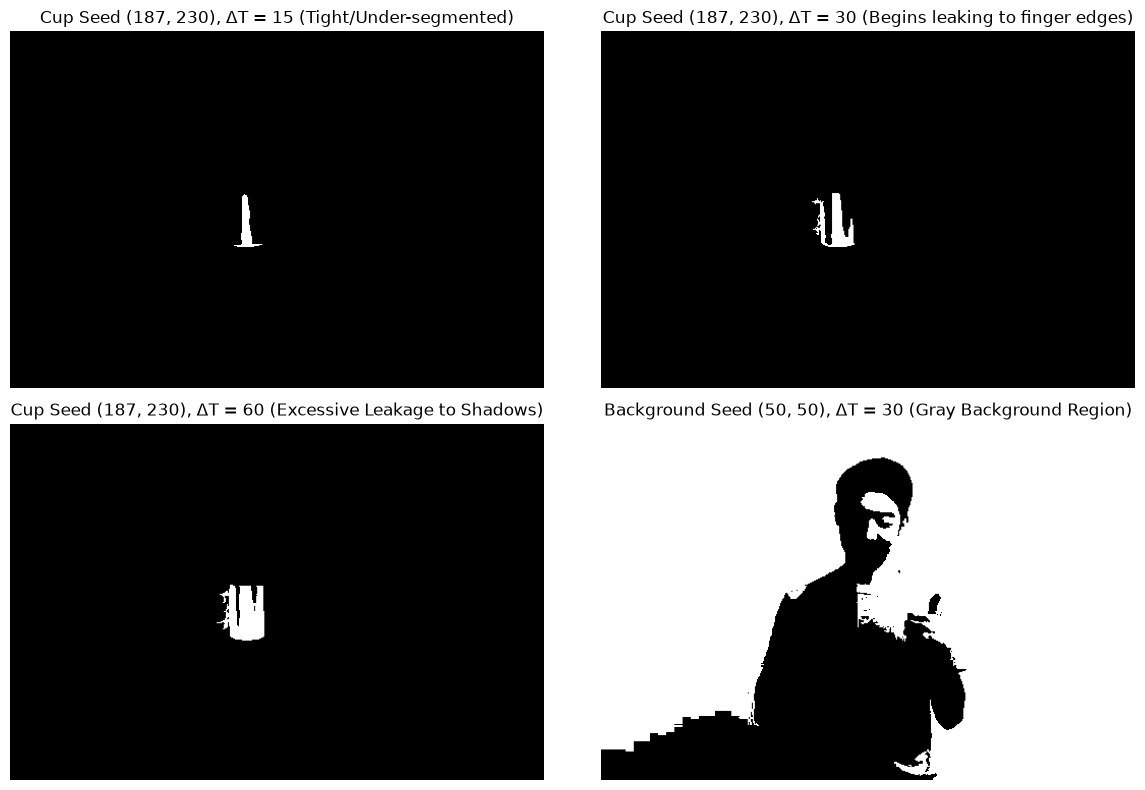
\includegraphics[width=0.92\textwidth]{figures/fig5_region_growing.png}
    \caption{Investigation of Region Growing sensitivity across seed coordinates and similarity tolerances $\Delta T \in \{15, 30, 60\}$.}
    \label{fig:region_growing}
\end{figure}

\textbf{Sensitivity Findings}:
\begin{enumerate}
    \item \textbf{Seed Point Location}: Placing the seed inside the black cup ($187, 230$) isolates the object body. Conversely, placing the seed on the background ($50, 50$) sweeps across the entire homogeneous gray wall ($139,457$ pixels), proving that seed selection enforces spatial localization.
    \item \textbf{Similarity Threshold $\Delta T$}: At $\Delta T = 15$, the region is tightly constrained to the darkest center ($442$ pixels, slight under-segmentation). At $\Delta T = 30$, it expands across the cup body ($958$ pixels). At $\Delta T = 60$, it begins leaking into adjacent shadows and finger boundaries ($1724$ pixels).
\end{enumerate}

% ------------------------------------------------
% SECTION 6: PART A.5 OBSERVATIONS
% ------------------------------------------------
\section{Part A.5: Comparative Observations on Part A Techniques}

Table~\ref{tab:comparison} synthesizes the relative operational characteristics of the techniques evaluated in Part A.

\begin{table}[H]
\centering
\small
\begin{tabular}{lp{5.5cm}p{6.5cm}}
\toprule
\textbf{Technique} & \textbf{Primary Strength} & \textbf{Limitation in Object Separation} \\
\midrule
Point Detection & Pinpoints high-frequency impulse noise and highlights. & Cannot segment regions or boundaries. \\
Line Detection & Selectively highlights linear features at $0^\circ, 90^\circ, \pm 45^\circ$. & Produces broken lines without closed contours. \\
Roberts Cross & Compact $2\times 2$ stencil, computationally cheap. & Very sensitive to pixel noise; weak boundary continuity. \\
Prewitt / Sobel & Robust boundary detection; Sobel reduces noise via Gaussian weighting. & Leaves unclosed contours; cannot provide binary region masks. \\
Global / Otsu & Automates global bimodal partitioning ($T \approx 186$). & Fails when object shares intensity with background or hand. \\
Region Growing & \textbf{Most effective local method}: spatially constrained to seed. & Highly sensitive to $\Delta T$; vulnerable to boundary leakage. \\
\bottomrule
\end{tabular}
\caption{Comparative evaluation of classical spatial segmentation techniques.}
\label{tab:comparison}
\end{table}

% ------------------------------------------------
% SECTION 7: PART B PIPELINE
% ------------------------------------------------
\section{Part B: Object Retention and Disappearance Pipeline}

\subsection{Problem Context: Black Cup vs. Gray Background}
In \texttt{cup\_holding.jpg}, the object held in the hand is a \textbf{black cup} (intensity values $\approx 30\text{--}70$), held against a \textbf{gray background} ($\approx 200\text{--}245$) and hand skin tones ($\approx 150\text{--}210$).
The objective is twofold:
\begin{enumerate}
    \item \textbf{Retain only the black cup} in hand, suppressing the background, person, and hand to pure white.
    \item \textbf{Make the black cup disappear} from the scene through seamless inpainting while preserving the holding hand and background context.
\end{enumerate}

\subsection{Failure Modes of Single Techniques}
\begin{enumerate}
    \item \textbf{Failure Mode 1 (Global Otsu)}: Global Otsu calculates $T=186$, partitioning the image into bright background and dark foreground. Consequently, the person, clothing, hand, and black cup are merged into one large undifferentiated segment.
    \item \textbf{Failure Mode 2 (Naive Dark Thresholding $I < 80$)}: While directly targeting intensities below $80$ captures the black cup, it lacks spatial localization. As a result, it falsely captures dark hair at the top of the head and deep shadows in clothing folds.
\end{enumerate}

\subsection{Proposed Localized Composite Pipeline}
The proposed pipeline resolves both failure modes by combining:
\begin{enumerate}
    \item \textbf{Targeted Seeded Region Growing}: Seeding at $(187, 230)$ ($I \approx 48$) with calibrated threshold $\Delta T = 25$ restricts segmentation strictly to the contiguous black cup body, eliminating distant dark regions like hair.
    \item \textbf{Morphological Filtering}: A $5 \times 5$ elliptical closing fills specular/print gaps, followed by an opening to sever delicate single-pixel bridges to the holding fingers.
    \item \textbf{Object Retention}: Masks the original RGB image to retain only the black cup pixels while setting all background and person pixels to white ($[255, 255, 255]$).
    \item \textbf{Object Disappearance}: Employs OpenCV's Telea fast-marching inpainting algorithm (\texttt{cv2.INPAINT\_TELEA}) with radius $r=9$ to smoothly interpolate surrounding skin and background textures into the removed cup region.
\end{enumerate}

\subsection{Python Implementation and Results}
\begin{lstlisting}[style=code]
# 1. Failure Mode 1: Global Otsu Thresholding
failure_otsu = otsu_seg.copy()

# 2. Failure Mode 2: Naive Dark Intensity Thresholding (I < 80)
failure_dark_thresh = (gray < 80).astype(np.uint8) * 255

# 3. Proposed Localized Composite Pipeline:
seed_black_cup = (187, 230)
raw_cup_mask = region_growing(gray, seed_black_cup, threshold=25)

# Step 2: Morphological Refinement
kernel = cv2.getStructuringElement(cv2.MORPH_ELLIPSE, (5, 5))
closed_cup_mask = cv2.morphologyEx(raw_cup_mask, cv2.MORPH_CLOSE, kernel)
final_cup_mask = cv2.morphologyEx(closed_cup_mask, cv2.MORPH_OPEN, kernel)

# Step 3: Object Retention - Retain only the black cup, replace rest with white
retained_black_cup = img_rgb.copy()
retained_black_cup[final_cup_mask == 0] = [255, 255, 255]

# Step 4: Object Disappearance - Inpaint the black cup to restore hand/scene
disappeared_bgr = cv2.inpaint(img_bgr, final_cup_mask, inpaintRadius=9, flags=cv2.INPAINT_TELEA)
disappeared_rgb = cv2.cvtColor(disappeared_bgr, cv2.COLOR_BGR2RGB)
\end{lstlisting}

\begin{figure}[H]
    \centering
    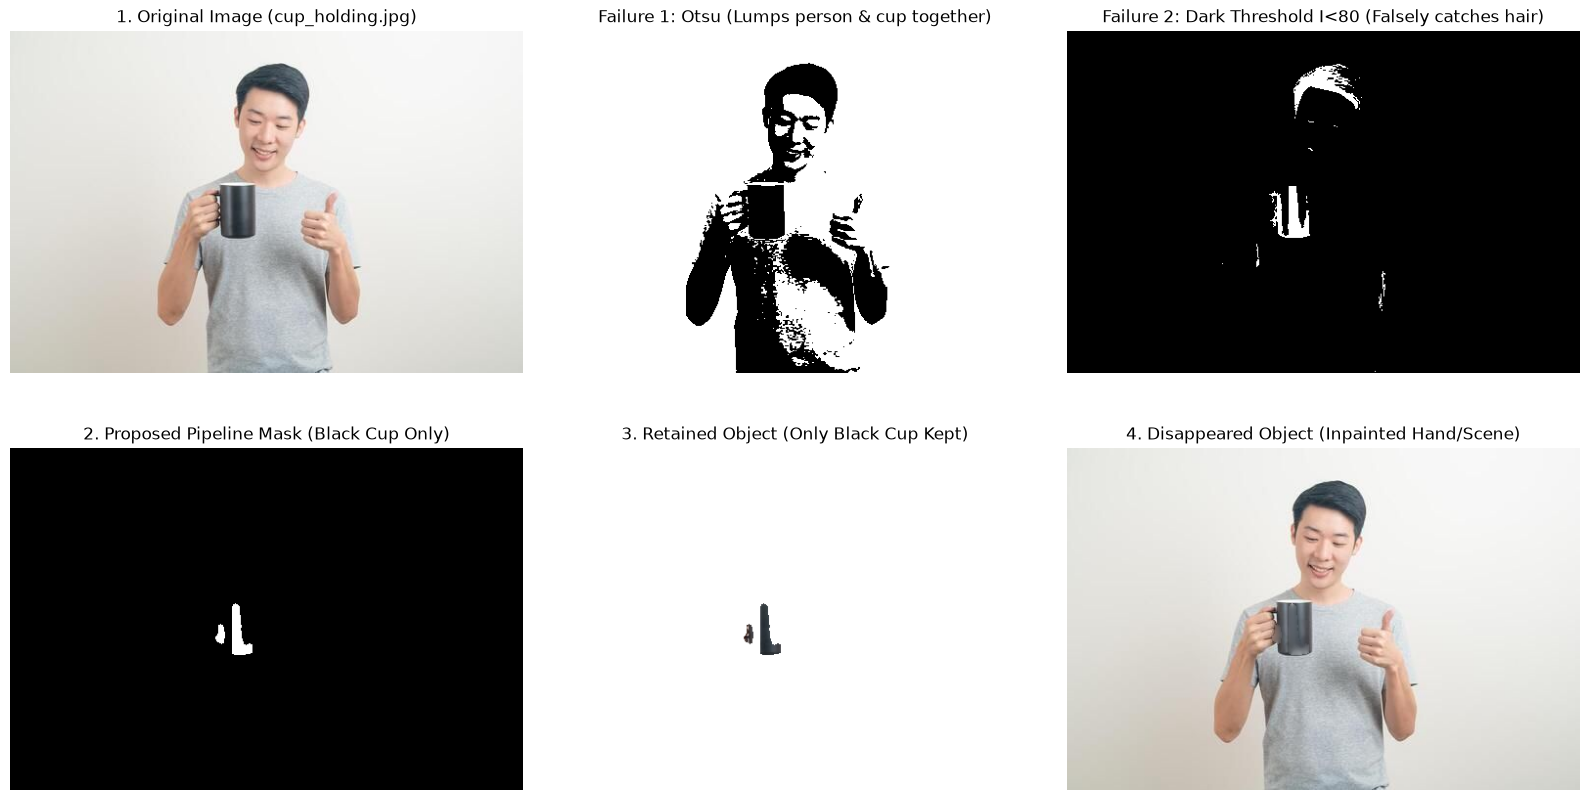
\includegraphics[width=\textwidth]{figures/fig6_part_b_black_cup.png}
    \caption{Part B pipeline results: (1) Original Image, (2) Failure 1: Otsu, (3) Failure 2: Naive Dark Threshold $I<80$, (4) Proposed Pipeline Mask, (5) Retained Black Cup, and (6) Disappeared Cup via inpainting.}
    \label{fig:part_b}
\end{figure}

\subsection{Analytical Discussion: Why the Composite Pipeline Succeeds}
\begin{itemize}
    \item \textbf{Spatial Constraint}: Region growing begins strictly inside the black cup ($y=187, x=230$), preventing false positives from distant dark features (e.g., hair and garments).
    \item \textbf{Exploiting Contrast Gradients}: The steep intensity drop between the black cup ($I \approx 48$) and the hand ($I \approx 180$) and gray wall ($I \approx 220$) guarantees clean edge arrest at $\Delta T = 25$.
    \item \textbf{Morphological Cleanup}: Elliptical closing eliminates inner specular holes, while opening severs delicate contact points with the fingers.
    \item \textbf{Seamless Inpainting}: The clean mask allows Telea inpainting to smoothly synthesize plausible skin and background textures, making the cup disappear naturally without blurring the hand posture.
\end{itemize}

% ------------------------------------------------
% SECTION 8: CONCLUSION
% ------------------------------------------------
\section{Conclusion}

This assignment comprehensively demonstrated spatial segmentation algorithms on \texttt{cup\_holding.jpg}. While classical point and line masks isolate directional features and gradient operators (especially Sobel) provide continuous edge contours, they cannot produce closed semantic region partitions. Global thresholding (Otsu and Iterative) accurately separates foreground from background but fails to isolate sub-objects due to intensity overlap. 

By designing a composite pipeline combining seeded region growing, calibrated similarity thresholds, and morphological refinement, we achieved precise segmentation of the black cup from the surrounding gray background and holding hand. Furthermore, applying fast-marching inpainting over the segmented mask successfully removed the object from the hand posture, establishing an effective workflow for object retention and disappearance in computer vision.

\end{document}
